% =============================================================================
% CAPÍTULO 2 - BLOQUE 2.6: ESTRATEGIAS AVANZADAS DE FRAGMENTACIÓN (CHUNKING),
% FORMULACIÓN GAUSSIANA SSIM, SELECCIÓN POR ENTROPÍA Y ALINEACIÓN AUDITIVA
% =============================================================================

\subsection{Estrategias Avanzadas de Fragmentación (\textit{Chunking}) y Alineación Temporal}
\label{subsec:chunking_alineacion}

\subsubsection{Obsolescencia de la Partición Fija, Detección de Planos y Agrupación de Escenas}
\label{subsubsec:obsolescencia_particion_fija}

El rendimiento, la precisión de recuperación y la viabilidad técnica de cualquier arquitectura de vectorización multimodal recaen, fundamentalmente, sobre su estrategia de partición de datos o \textit{chunking} \cite{adaptive_chunking2026, multi_rag2025}. %
Indexar las pistas de audio, los subtítulos y las secuencias de fotogramas de vídeo de forma desincronizada o mediante divisiones temporales arbitrarias destruye por completo la cohesión semántica y cronológica del documento multimedia \cite{mixpeek_chunking}. %[cite: 5]

La metodología de fragmentación más elemental —consistente en cortar un archivo de vídeo en intervalos regulares y rígidos, por ejemplo, cada $5$ o $10$ segundos— constituye un enfoque obsoleto en el estado del arte de 2026 \cite{video_rac2025, mixpeek_chunking}. %[cite: 3, 5]
Aplicar una rejilla temporal ciega produce invariablemente cortes abruptos en mitad de una oración hablada, interrumpe un cambio de plano cinematográfico o divide en dos fragmentos inconexos la transición de una diapositiva académica o la escritura de un bloque de código \cite{video_rac2025, mixpeek_chunking}. %[cite: 3, 5]
Forzar posteriormente al modelo de \textit{embeddings} o al modelo generativo a interpretar fragmentos visuales mutilados introduce un ruido contextual severo que degrada las métricas de relevancia y fidelidad \cite{video_rac2025}. %[cite: 5]

Para erradicar esta fragmentación destructiva, las arquitecturas contemporáneas aplican algoritmos de \textbf{detección de límites de plano (\textit{shot boundary detection})} acoplados a procesamiento paralelo profundo \cite{mixpeek_chunking}. %[cite: 3, 5]
Estos algoritmos evalúan fotograma a fotograma la continuidad visual midiendo bien la divergencia de histogramas en espacios de color robustos ante variaciones de iluminación —como el espacio HSV (\textit{Hue, Saturation, Value}), donde un parpadeo de cámara afecta al canal de valor pero no altera el matiz cromático—, o bien la similitud estructural (SSIM) entre fotogramas secuenciales, garantizando que cada \textit{chunk} represente una unidad narrativa o visualmente coherente \cite{mixpeek_chunking, video_rac2025}. %[cite: 3, 5]

Por otra parte, cuando el vídeo presenta cortes de cámara muy rápidos y la granularidad del plano resultante es excesivamente fina, la literatura incorpora técnicas de \textbf{agrupación de escenas (\textit{scene grouping})} \cite{mixpeek_chunking}. %[cite: 5]
Este procedimiento fusiona planos consecutivos cuyas representaciones vectoriales preliminares superan un umbral de similitud predefinido, condensando múltiples micro-planos en intervalos temporales más largos y semánticamente estables antes de su indexación definitiva \cite{mixpeek_chunking}. %[cite: 5]

La Figura~\ref{fig:fixed_vs_adaptive_videorac} contrasta el efecto destructivo de la partición por intervalos fijos frente a la preservación de unidades narrativas mediante detección adaptativa de límites de plano y agrupación de escenas. %[cite: 3, 5]

\begin{figure}[htbp]
\centering
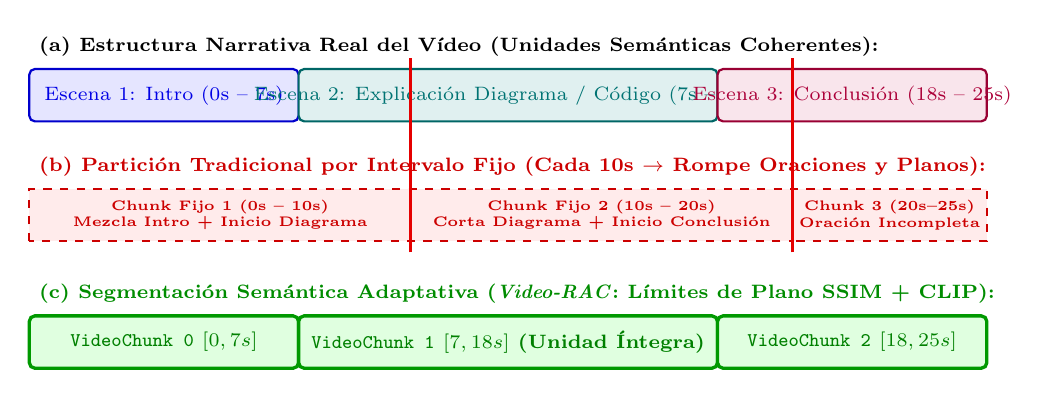
\begin{tikzpicture}[scale=0.95]
% Flujo Real de Eventos en el Vídeo
\node[font=\scriptsize\bfseries, anchor=west] at (0, 3.3) {(a) Estructura Narrativa Real del Vídeo (Unidades Semánticas Coherentes):};
\draw[fill=blue!10, draw=blue!80!black, thick, rounded corners=2pt] (0, 2.3) rectangle (3.6, 3.0);
\node[font=\scriptsize, blue!90!black] at (1.8, 2.65) {Escena 1: Intro (0s -- 7s)};

\draw[fill=teal!12, draw=teal!80!black, thick, rounded corners=2pt] (3.6, 2.3) rectangle (9.2, 3.0);
\node[font=\scriptsize, teal!90!black] at (6.4, 2.65) {Escena 2: Explicación Diagrama / Código (7s -- 18s)};

\draw[fill=purple!10, draw=purple!80!black, thick, rounded corners=2pt] (9.2, 2.3) rectangle (12.8, 3.0);
\node[font=\scriptsize, purple!90!black] at (11.0, 2.65) {Escena 3: Conclusión (18s -- 25s)};

% Partición Fija (Obsoleta)
\node[font=\scriptsize\bfseries, red!80!black, anchor=west] at (0, 1.7) {(b) Partición Tradicional por Intervalo Fijo (Cada 10s $\to$ Rompe Oraciones y Planos):};
\draw[fill=red!8, draw=red!80!black, thick, dashed] (0, 0.7) rectangle (5.1, 1.4);
\node[font=\tiny\bfseries, red!80!black, align=center] at (2.55, 1.05) {Chunk Fijo 1 (0s -- 10s)\\Mezcla Intro + Inicio Diagrama};

\draw[fill=red!8, draw=red!80!black, thick, dashed] (5.1, 0.7) rectangle (10.2, 1.4);
\node[font=\tiny\bfseries, red!80!black, align=center] at (7.65, 1.05) {Chunk Fijo 2 (10s -- 20s)\\Corta Diagrama + Inicio Conclusión};

\draw[fill=red!8, draw=red!80!black, thick, dashed] (10.2, 0.7) rectangle (12.8, 1.4);
\node[font=\tiny\bfseries, red!80!black, align=center] at (11.5, 1.05) {Chunk 3 (20s--25s)\\Oración Incompleta};

% Líneas de corte erróneas
\draw[very thick, red!90!black] (5.1, 0.55) -- (5.1, 3.15);
\draw[very thick, red!90!black] (10.2, 0.55) -- (10.2, 3.15);

% Segmentación Semántica Adaptativa (Video-RAC)
\node[font=\scriptsize\bfseries, green!55!black, anchor=west] at (0, 0.0) {(c) Segmentación Semántica Adaptativa (\textit{Video-RAC}: Límites de Plano SSIM + CLIP):};
\draw[fill=green!12, draw=green!60!black, very thick, rounded corners=2pt] (0, -1.0) rectangle (3.6, -0.3);
\node[font=\scriptsize\bfseries, green!50!black] at (1.8, -0.65) {\texttt{VideoChunk 0} $[0, 7\text{s}]$};

\draw[fill=green!12, draw=green!60!black, very thick, rounded corners=2pt] (3.6, -1.0) rectangle (9.2, -0.3);
\node[font=\scriptsize\bfseries, green!50!black] at (6.4, -0.65) {\texttt{VideoChunk 1} $[7, 18\text{s}]$ (Unidad Íntegra)};

\draw[fill=green!12, draw=green!60!black, very thick, rounded corners=2pt] (9.2, -1.0) rectangle (12.8, -0.3);
\node[font=\scriptsize\bfseries, green!50!black] at (11.0, -0.65) {\texttt{VideoChunk 2} $[18, 25\text{s}]$};
\end{tikzpicture}
\caption{Comparativa estructural entre (b) la división arbitraria en intervalos fijos, que introduce ruido contextual al cortar escenas y oraciones a la mitad, y (c) la segmentación semántica adaptativa (\textit{Video-RAC}), que alinea exactamente los límites de cada \texttt{VideoChunk} con las transiciones reales del contenido \cite{video_rac2025, mixpeek_chunking}.} %[cite: 3, 5]
\label{fig:fixed_vs_adaptive_videorac}
\end{figure}

\subsubsection{Metodología Híbrida \textit{Video-RAC} y Formulación Matemática del SSIM Gaussiano}
\label{subsubsec:metodologia_videorac_ssim}

Dentro del ámbito de los vídeos educativos, académicos y tutoriales técnicos, la arquitectura \textbf{Video-RAC (\textit{Retrieval Adaptive Chunking})} se ha consolidado como el estándar metodológico de referencia \cite{video_rac2025}. %[cite: 3, 5]
\textit{Video-RAC} abandona las particiones estáticas en favor de un criterio híbrido que evalúa cada transición temporal combinando la similitud del coseno de \textit{embeddings} visuales ligeros generados por CLIP con el Índice de Similitud Estructural (SSIM) \cite{video_rac2025}. %[cite: 3, 5]

Específicamente, la formulación teórica de \textit{Video-RAC} emplea el modelo \texttt{openai/clip-vit-base-patch32} para extraer representaciones rápidas de los fotogramas consecutivos $F_t$ y $F_{t+1}$, ponderando su similitud semántica con la similitud estructural mediante un factor de balance $\alpha = 0,6$ \cite{video_rac2025}: %[cite: 5]

\begin{equation}
S_{\text{híbrida}}(F_t, F_{t+1}) = \alpha \cdot \cos\!\left(\mathbf{e}_{\text{CLIP}}(F_t), \, \mathbf{e}_{\text{CLIP}}(F_{t+1})\right) + (1 - \alpha) \cdot \text{SSIM}(F_t, F_{t+1})
\label{eq:videorac_hibrido}
\end{equation} %[cite: 5]

Los hiperparámetros canónicos reportados en la literatura para determinar dónde concluye una unidad semántica y comienza la siguiente estipulan un factor de balance $\alpha = 0,6$, un umbral de similitud de \textit{embeddings} CLIP de $\tau_{\text{CLIP}} = 0,85$ y un umbral estructural de $\tau_{\text{SSIM}} = 0,80$ \cite{video_rac2025}. %[cite: 5]

En implementaciones de producción optimizadas para ejecutarse localmente en CPU sin requerir la carga de pesos adicionales de CLIP durante el preprocesamiento (tal y como se implementa en el módulo \texttt{src/processing/video\_chunker.py}), la detección de límites de plano se resuelve directamente mediante la formulación matemática exacta del \textbf{Índice de Similitud Estructural (SSIM)} con ventana Gaussiana en OpenCV. %[cite: 3]
Dados dos fotogramas consecutivos convertidos a escala de grises y redimensionados a un ancho de análisis rápido (\texttt{resize\_width = 160} píxeles para la fase de corte), representados como matrices en coma flotante de doble precisión $a, b \in \mathbb{R}^{H \times W}$ (\texttt{np.float64}), el algoritmo aplica un filtro de desenfoque Gaussiano bidimensional \texttt{cv2.GaussianBlur} con tamaño de núcleo impar $K \times K$ (\texttt{window\_size = 7}) y desviación estándar $\sigma = 1,5$ para obtener las medias locales $\mu_a, \mu_b$: %[cite: 3]

\begin{equation}
\mu_a = G_{K \times K, \, \sigma=1.5} * a, \qquad \mu_b = G_{K \times K, \, \sigma=1.5} * b
\label{eq:ssim_medias_locales}
\end{equation} %[cite: 3]

A partir de los cuadrados de las medias ($\mu_a^2, \mu_b^2$) y de su producto cruzado ($\mu_{ab} = \mu_a \mu_b$), las varianzas locales $\sigma_a^2, \sigma_b^2$ y la covarianza cruzada local $\sigma_{ab}$ se calculan matricialmente mediante convolución Gaussiana como: %[cite: 3]

\begin{equation}
\sigma_a^2 = \left(G_{K \times K, \, \sigma=1.5} * (a \odot a)\right) - \mu_a^2, \quad
\sigma_b^2 = \left(G_{K \times K, \, \sigma=1.5} * (b \odot b)\right) - \mu_b^2, \quad
\sigma_{ab} = \left(G_{K \times K, \, \sigma=1.5} * (a \odot b)\right) - \mu_{ab}
\label{eq:ssim_varianzas_covarianza}
\end{equation} %[cite: 3]

donde $\odot$ denota el producto elemento a elemento (\textit{Hadamard product}). %[cite: 3]
Con estas matrices estadísticas e introduciendo las constantes de estabilidad numérica para un rango dinámico de 8 bits ($L = 255$), definidas como $C_1 = (0,01 \times 255)^2 = 6,5025$ y $C_2 = (0,03 \times 255)^2 = 58,5225$, el mapa espacial SSIM y su escalar medio resultante en el rango $[-1, 1]$ vienen dados por: %[cite: 3]

\begin{equation}
\text{SSIM}_{\text{map}}(a, b) = \frac{(2\mu_{ab} + C_1)(2\sigma_{ab} + C_2)}{(\mu_a^2 + \mu_b^2 + C_1)(\sigma_a^2 + \sigma_b^2 + C_2)}, \qquad
\overline{\text{SSIM}}(a, b) = \frac{1}{H \cdot W} \sum_{y=1}^{H} \sum_{x=1}^{W} \text{SSIM}_{\text{map}}(y, x)
\label{eq:ssim_mapa_y_media}
\end{equation} %[cite: 3]

Cuando el valor escalar $\overline{\text{SSIM}}(a, b)$ cae por debajo del umbral configurado (\texttt{threshold}, calibrado entre $0,50$ y $0,80$) y el número de fotogramas acumulados desde el corte anterior iguala o supera el mínimo permitido (\texttt{min\_shot\_frames = 12} a $45$ fotogramas para filtrar destellos luminosos espurios), la función \texttt{detect\_shot\_boundaries} consolida e instancia un objeto inmutable \texttt{VideoChunk(index, start\_frame, end\_frame, start\_time, end\_time)}. %[cite: 3]

La Figura~\ref{fig:pipeline_ssim_opencv} detalla este flujo de cálculo matricial implementado en \texttt{compute\_ssim} y \texttt{detect\_shot\_boundaries}. %[cite: 3]

\begin{figure}[htbp]
\centering
\begin{tikzpicture}[
    node distance=0.45cm and 0.65cm,
    matbox/.style={rectangle, draw=black!80, fill=gray!10, thick, minimum width=2.7cm, minimum height=0.95cm, align=center, font=\scriptsize, rounded corners=2pt},
    blurbox/.style={rectangle, draw=blue!80!black, fill=blue!8, thick, minimum width=3.2cm, minimum height=1.1cm, align=center, font=\scriptsize, rounded corners=2pt},
    mapnode/.style={rectangle, draw=purple!80!black, fill=purple!8, thick, minimum width=3.3cm, minimum height=1.1cm, align=center, font=\scriptsize, rounded corners=2pt},
    decnode/.style={diamond, aspect=2.1, draw=orange!85!black, fill=orange!12, very thick, minimum width=2.8cm, minimum height=1.1cm, align=center, font=\scriptsize\bfseries},
    chunkbox/.style={rectangle, draw=green!60!black, fill=green!12, very thick, minimum width=2.9cm, minimum height=1.1cm, align=center, font=\scriptsize\bfseries, rounded corners=2pt},
    arrow/.style={-stealth, thick, draw=black!80}
]
\node[matbox] (frames) at (-5.3, 0.0) {Par Consecutivo\\$F_{t-1}, F_t$ (Grises)\\ \texttt{float64} ($160\text{ px}$)};

\node[blurbox] (gauss) at (-1.8, 0.0) {\texttt{cv2.GaussianBlur}\\Núcleo $7\times 7, \, \sigma = 1,5$\\$\mu_a, \mu_b, \sigma_a^2, \sigma_b^2, \sigma_{ab}$};

\node[mapnode] (ssim) at (1.9, 0.0) {Mapa $\text{SSIM}_{\text{map}}$\\($C_1, C_2$ con $L=255$)\\Media: \texttt{ssim\_map.mean()}};

\node[decnode] (cut) at (1.9, -2.0) {¿$\overline{\text{SSIM}} < \tau$\\y $\Delta f \ge f_{\min}$?};

\node[chunkbox] (out) at (5.6, -2.0) {Emite \texttt{VideoChunk}\\(\texttt{start\_frame}, \texttt{end\_frame},\\ \texttt{start\_time}, \texttt{end\_time})};

\node[matbox, minimum width=2.7cm] (cont) at (-2.1, -2.0) {Continúa Plano Actual\\Acumula Fotograma $F_t$};

\draw[arrow] (frames) -- (gauss);
\draw[arrow] (gauss) -- (ssim);
\draw[arrow] (ssim) -- (cut);
\draw[arrow, draw=green!60!black] (cut) -- node[above, font=\scriptsize\bfseries, green!60!black] {Sí (Corte)} (out);
\draw[arrow, draw=blue!80!black] (cut) -- node[above, font=\scriptsize\bfseries, blue!80!black] {No} (cont);
\end{tikzpicture}
\caption{Flujo algorítmico del cálculo del Índice de Similitud Estructural (SSIM) mediante filtrado Gaussiano en OpenCV (\texttt{compute\_ssim}) y criterio de consolidación de objetos \texttt{VideoChunk} en \texttt{detect\_shot\_boundaries}.} %[cite: 3]
\label{fig:pipeline_ssim_opencv}
\end{figure}

\subsubsection{Selección de Fotogramas Clave mediante Entropía Matemática de Shannon}
\label{subsubsec:seleccion_entropia_shannon}

Una vez que el vídeo ha sido particionado en unidades semánticamente coherentes (\texttt{VideoChunk}), enviar la totalidad de los fotogramas de cada fragmento (a razón de $30$ o $60$ fotogramas por segundo) hacia la API del modelo de \textit{embeddings} resultaría computacional y económicamente inviable \cite{video_rac2025, gemini_emb2_docs}. %[cite: 3]
Para comprimir el volumen visual sin perder el contenido informativo del plano, la metodología \textit{Video-RAC} establece una estrategia de \textbf{selección de fotogramas por entropía} implementada en la función \texttt{extract\_key\_frames} \cite{video_rac2025}. %[cite: 3]

Para cada objeto \texttt{VideoChunk} delimitado entre los índices de fotograma $[f_{\text{ini}}, f_{\text{fin}}]$, el algoritmo selecciona exactamente tres fotogramas representativos ordenados cronológicamente \cite{video_rac2025}: %[cite: 3]
\begin{enumerate}
    \item \textbf{Fotograma Inicial ($F_{f_{\text{ini}}}$):} Captura el estado visual de partida del evento al abrirse el plano. %[cite: 3]
    \item \textbf{Fotograma Intermedio de Máxima Entropía ($F_{f^*}$):} De entre los fotogramas interiores $t \in (f_{\text{ini}}, f_{\text{fin}})$ (evaluados de forma exhaustiva o mediante un paso de muestreo \texttt{entropy\_step}), se selecciona aquel que maximiza la \textbf{Entropía de Información de Shannon} $H(F_t)$, la cual cuantifica la riqueza y densidad de detalle visual (por ejemplo, el instante en que un diagrama o bloque de código está completamente desplegado en pantalla y no oculto o en transición). %[cite: 3]
    \item \textbf{Fotograma Final ($F_{f_{\text{fin}}}$):} Registra el estado consolidado del plano justo antes del corte hacia la siguiente escena. %[cite: 3]
\end{enumerate}

Matemáticamente, para calcular la entropía de Shannon de un fotograma candidato $F_t$ convertido a escala de grises con $L = 256$ niveles de intensidad ($i \in \{0, 1, \dots, 255\}$), se obtiene primero su histograma de frecuencias absolutas $h(i)$ mediante \texttt{cv2.calcHist} y se normaliza por el número total de píxeles $N_{\text{pix}} = H \times W$ para obtener la distribución de probabilidad discreta $p_i = h(i) / N_{\text{pix}}$: %[cite: 3]

\begin{equation}
H(F_t) = -\sum_{\substack{i=0 \\ p_i > 0}}^{255} p_i \log_2(p_i), \qquad f^* = \arg\max_{t \in (f_{\text{ini}}, \, f_{\text{fin}})} H(F_t)
\label{eq:entropia_shannon_keyframe}
\end{equation} %[cite: 3]

La Figura~\ref{fig:seleccion_entropia_shannon} ilustra la evolución de la curva de entropía $H(F_t)$ dentro de los límites de un \texttt{VideoChunk} y la extracción de la terna de matrices NumPy que alimenta al vectorizador multimodal. %[cite: 3]

\begin{figure}[htbp]
\centering
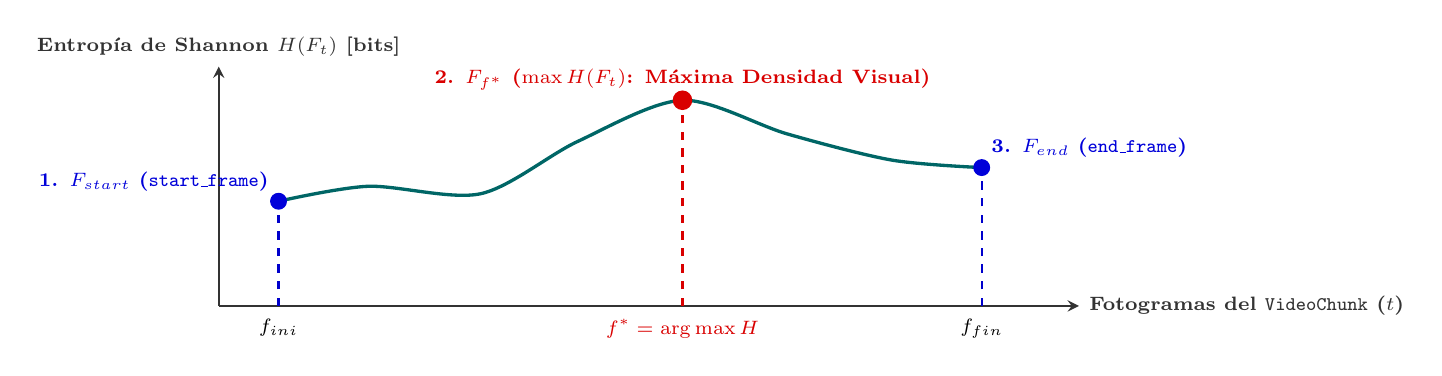
\begin{tikzpicture}[scale=0.95]
% Ejes de la gráfica de entropía
\draw[-stealth, thick, black!80] (0,0) -- (11.5,0) node[right, font=\scriptsize\bfseries] {Fotogramas del \texttt{VideoChunk} ($t$)};
\draw[-stealth, thick, black!80] (0,0) -- (0,3.2) node[above, font=\scriptsize\bfseries] {Entropía de Shannon $H(F_t)$ [bits]};

% Líneas de inicio, máximo y fin
\draw[dashed, blue!80!black, thick] (0.8, 0) -- (0.8, 1.4);
\draw[dashed, red!85!black, very thick] (6.2, 0) -- (6.2, 2.75);
\draw[dashed, blue!80!black, thick] (10.2, 0) -- (10.2, 1.85);

% Curva de entropía simulada dentro del chunk
\draw[very thick, teal!80!black] plot [smooth] coordinates {
    (0.8, 1.4) (2.0, 1.6) (3.5, 1.5) (4.8, 2.2) (6.2, 2.75) (7.6, 2.3) (9.0, 1.95) (10.2, 1.85)
};

% Puntos seleccionados
\filldraw[blue!85!black] (0.8, 1.4) circle (3pt) node[above left, font=\scriptsize\bfseries] {1. $F_{\text{start}}$ (\texttt{start\_frame})};
\filldraw[red!85!black] (6.2, 2.75) circle (3.5pt) node[above, font=\scriptsize\bfseries] {2. $F_{f^*}$ ($\max H(F_t)$: Máxima Densidad Visual)};
\filldraw[blue!85!black] (10.2, 1.85) circle (3pt) node[above right, font=\scriptsize\bfseries] {3. $F_{\text{end}}$ (\texttt{end\_frame})};

% Etiquetas en el eje X
\node[below, font=\scriptsize] at (0.8, -0.05) {$f_{\text{ini}}$};
\node[below, font=\scriptsize\bfseries, red!85!black] at (6.2, -0.05) {$f^* = \arg\max H$};
\node[below, font=\scriptsize] at (10.2, -0.05) {$f_{\text{fin}}$};
\end{tikzpicture}
\caption{Selección de fotogramas clave basada en Entropía de Shannon (\texttt{extract\_key\_frames}) según la metodología \textit{Video-RAC}: extracción del fotograma inicial, el fotograma final y el fotograma intermedio que maximiza la densidad de información visual $H(F_t)$ \cite{video_rac2025}.} %[cite: 3]
\label{fig:seleccion_entropia_shannon}
\end{figure}

\subsubsection{Alineación Forzada del Audio (\textit{Forced Alignment}), Silero VAD y Diarización de Hablantes}
\label{subsubsec:alineacion_forzada_audio}

En paralelo a la segmentación visual, la dimensión auditiva exige una ingeniería de fragmentación igualmente rigurosa \cite{mixpeek_chunking, whisperx_silero}. %[cite: 4, 5]
El estado del arte descarta por completo las transcripciones planas carentes de marcas de tiempo y establece una canalización acústica en cuatro etapas implementada en torno al módulo \texttt{src/processing/audio\_transcriber.py} \cite{mixpeek_chunking, whisperx_silero}: %[cite: 3, 4, 5]

\begin{enumerate}
    \item \textbf{Extracción de Pista Acústica:} A partir del contenedor de vídeo original (\texttt{.mp4}), se desmultiplexa la señal de audio hacia un archivo temporal sin compresión o de alta fidelidad (\texttt{.wav} o \texttt{.mp3}) empleando herramientas de bajo nivel como \texttt{ffmpeg} o \texttt{moviepy} ejecutadas de forma no bloqueante (\texttt{asyncio.to\_thread}). %[cite: 3, 4]
    \item \textbf{Detección de Actividad de Voz (\textit{Voice Activity Detection} -- Silero VAD):} Antes de invocar al modelo de transcripción, el flujo de audio se filtra mediante redes ultraligeras de detección de voz como \textbf{Silero VAD}, la cual cuenta con aproximadamente \textbf{un millón de parámetros} y ofrece una ejecución ultrarrápida en CPU para aislar los segmentos de discurso humano respecto del silencio y del ruido ambiental, evitando alucinaciones fonéticas del modelo ASR durante pausas acústicas \cite{whisperx_silero, mixpeek_chunking}. %[cite: 5]
    \item \textbf{Transcripción Fonética, Alineación Forzada (\textit{WhisperX}) y Diarización:} Los segmentos con voz activa se procesan mediante motores de reconocimiento avanzado como \textbf{Whisper}, acoplados a algoritmos de \textbf{alineación forzada} como \textbf{WhisperX} o \textbf{Montreal Forced Aligner} \cite{whisperx_silero, mixpeek_chunking}. %[cite: 4, 5]
    Este acoplamiento genera transcripciones con precisión a nivel de palabra y fonema, vinculando cada término exacto con su marca de tiempo en milisegundos $[t_{\text{ini}}^{\text{aud}}, t_{\text{fin}}^{\text{aud}}]$, mientras que la etapa de \textbf{diarización de hablantes} etiqueta acústicamente cada bloque textual con la identidad del interlocutor \cite{mixpeek_chunking}. %[cite: 5]
    \item \textbf{Superposición y Acoplamiento con \texttt{VideoChunk} (\texttt{align\_transcript\_with\_chunks}):} Finalmente, los segmentos transcritos se proyectan sobre los intervalos temporales $[t_{\text{start}}^{(i)}, t_{\text{end}}^{(i)}]$ de los objetos \texttt{VideoChunk} generados previamente por la etapa visual (CLIP/SSIM) \cite{mixpeek_chunking}. %[cite: 3, 4, 5]
\end{enumerate}

Formalmente, dado un \texttt{VideoChunk} visual $C_i$ con intervalo $[t_{\text{start}}^{(i)}, t_{\text{end}}^{(i)}]$ y una lista de segmentos de transcripción auditiva $S_j = (\tau_{\text{ini}}^{(j)}, \tau_{\text{fin}}^{(j)}, \text{texto}_j)$, la condición matemática de intersección temporal $\Delta \tau_{i,j}$ que determina la asignación o concatenación del texto en el atributo \texttt{VideoChunk.transcript} viene dada por: %[cite: 3, 4]

\begin{equation}
\Delta \tau_{i,j} = \max\!\left(0, \, \min\!\left(t_{\text{end}}^{(i)}, \, \tau_{\text{fin}}^{(j)}\right) - \max\!\left(t_{\text{start}}^{(i)}, \, \tau_{\text{ini}}^{(j)}\right)\right) > 0
\label{eq:solapamiento_audio_video}
\end{equation} %[cite: 3, 4]

La Figura~\ref{fig:alineacion_forzada_audio_video} muestra la arquitectura completa de esta canalización paralela visual y auditiva, garantizando que al recuperar un fragmento el sistema disponga simultáneamente de los fotogramas clave, la transcripción exacta pronunciada en ese segundo y la identidad del hablante \cite{mixpeek_chunking}. %[cite: 3, 4, 5]

\begin{figure}[htbp]
\centering
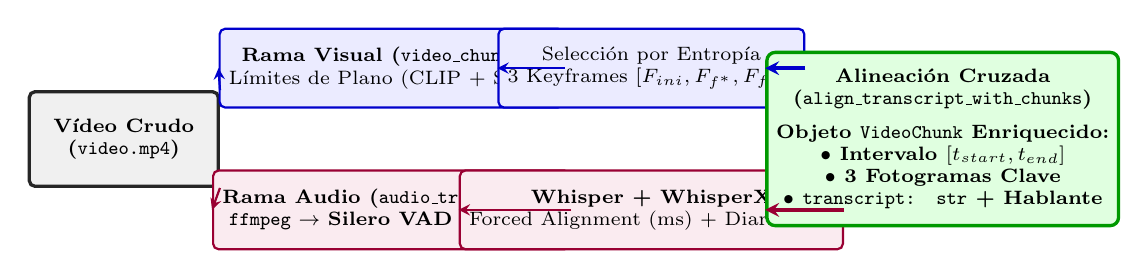
\begin{tikzpicture}[
    node distance=0.45cm and 0.6cm,
    srcnode/.style={rectangle, draw=black!85, fill=gray!12, very thick, minimum width=2.4cm, minimum height=1.2cm, align=center, font=\scriptsize\bfseries, rounded corners=2pt},
    visnode/.style={rectangle, draw=blue!80!black, fill=blue!8, thick, minimum width=2.8cm, minimum height=1.0cm, align=center, font=\scriptsize, rounded corners=2pt},
    audnode/.style={rectangle, draw=purple!80!black, fill=purple!8, thick, minimum width=2.8cm, minimum height=1.0cm, align=center, font=\scriptsize, rounded corners=2pt},
    alignbox/.style={rectangle, draw=green!60!black, fill=green!12, very thick, minimum width=3.3cm, minimum height=2.2cm, align=center, font=\scriptsize\bfseries, rounded corners=3pt},
    arrow/.style={-stealth, thick, draw=black!80}
]
% Entrada común
\node[srcnode] (mp4) at (-5.4, 0.0) {Vídeo Crudo\\(\texttt{video.mp4})};

% Rama Superior: Canal Visual
\node[visnode] (ssim) at (-2.0, 0.9) {\textbf{Rama Visual (\texttt{video\_chunker})}\\Límites de Plano (CLIP + SSIM)};
\node[visnode] (ent) at (1.3, 0.9) {Selección por Entropía\\3 Keyframes $[F_{\text{ini}}, F_{f^*}, F_{\text{fin}}]$};

% Rama Inferior: Canal Auditivo
\node[audnode] (vad) at (-2.0, -0.9) {\textbf{Rama Audio (\texttt{audio\_transcriber})}\\ \texttt{ffmpeg} $\to$ \textbf{Silero VAD} (1M par.)};
\node[audnode] (whisp) at (1.3, -0.9) {\textbf{Whisper + WhisperX}\\Forced Alignment (ms) + Diarización};

% Nodo de Fusión / Alineación Temporal
\node[alignbox] (out) at (5.0, 0.0) {\textbf{Alineación Cruzada}\\(\texttt{align\_transcript\_with\_chunks})\\[4pt]
Objeto \texttt{VideoChunk} Enriquecido:\\
$\bullet$ Intervalo $[t_{\text{start}}, t_{\text{end}}]$\\
$\bullet$ 3 Fotogramas Clave\\
$\bullet$ \texttt{transcript: str} + Hablante};

\draw[arrow, blue!80!black] (mp4.north east) -- (ssim.west);
\draw[arrow, blue!80!black] (ssim.east) -- (ent.west);
\draw[arrow, blue!80!black, very thick] (ent.east) -- (out.west |- ent.east);

\draw[arrow, purple!80!black] (mp4.south east) -- (vad.west);
\draw[arrow, purple!80!black] (vad.east) -- (whisp.west);
\draw[arrow, purple!80!black, very thick] (whisp.east) -- (out.west |- whisp.east);
\end{tikzpicture}
\caption{Arquitectura de procesamiento paralelo y alineación forzada intermodal: la rama visual segmenta el vídeo mediante CLIP/SSIM y extrae tres fotogramas por entropía de Shannon, mientras la rama auditiva filtra silencios con Silero VAD y alinea las marcas de tiempo de WhisperX sobre cada \texttt{VideoChunk} \cite{video_rac2025, whisperx_silero, mixpeek_chunking}.} %[cite: 3, 4, 5]
\label{fig:alineacion_forzada_audio_video}
\end{figure}

El Cuadro~\ref{tab:parametros_chunking_audio} resume todos los parámetros matemáticos y algorítmicos que gobiernan las etapas de fragmentación visual y alineación auditiva descritas en esta sección. %[cite: 3, 4, 5]

\begin{table}[htbp]
\centering
\caption{Especificaciones técnicas de la estrategia de fragmentación semántica adaptativa (\textit{Video-RAC}) y alineación forzada de audio \cite{video_rac2025, whisperx_silero, mixpeek_chunking}.} %[cite: 3, 4, 5]
\label{tab:parametros_chunking_audio}
\begin{tabular}{llll}
\hline
\textbf{Componente / Parámetro} & \textbf{Modelo / Algoritmo} & \textbf{Valor de Referencia} & \textbf{Función en el Pipeline} \\
\hline
Codificador visual híbrido & \texttt{clip-vit-base-patch32} & $\alpha = 0,6$, $\tau_{\text{CLIP}} = 0,85$ & Similitud semántica entre planos (\textit{Video-RAC}) \\
Índice estructural local & SSIM Gaussiano (OpenCV) & $\tau_{\text{SSIM}} = 0,80$ (o $0,5\text{--}0,8$) & Detección de bordes de plano ($K=7, \, \sigma=1,5$) \\
Constantes de estabilidad & Rango dinámico $L = 255$ & $C_1 = 6,50, \, C_2 = 58,52$ & Evita división por cero en zonas oscuras \\
Filtro de planos espurios & \texttt{min\_shot\_frames} & $12$ a $45$ fotogramas & Descarta parpadeos menores a $0,5\text{--}1,5\text{ s}$ \\
Muestreo de fotogramas & Entropía de Shannon $H(F_t)$ & $3$ frames (\texttt{ini}, $\max H$, \texttt{fin}) & Máxima densidad visual por \texttt{VideoChunk} \\
Detección de voz activa & Silero VAD (CPU) & $\sim 10^6$ parámetros (1M) & Aísla discurso humano de silencio y ruido \\
Alineación y diarización & Whisper + WhisperX / MFA & Precisión en milisegundos & Anclaje palabra a palabra e identidad hablante \\
\hline
\end{tabular}
\end{table}